%  DOCUMENT CLASS
\documentclass[a4paper,12pt,twoside]{scrreprt}

%PACKAGES
\usepackage[latin1]{inputenc}  % Quelltext ist ISO-8859-1 codiert
\usepackage[ngerman]{babel}
\usepackage[reqno,fleqn]{amsmath}
\setlength\mathindent{10mm}
\usepackage{amssymb}
\usepackage{amsthm}
\usepackage{amsfonts}
%\usepackage{extarrows}
\usepackage{fancyhdr}
\usepackage{units}
\usepackage{fourier, eurosym}
\usepackage{syntax}
\usepackage{graphicx}
\usepackage{color}
\usepackage{colortbl}
\definecolor{dunkelgrau}{rgb}{0.7,0.7,0.7}

% FORMATIERUNG
\usepackage[paper=a4paper,left=30mm,right=25mm,top=30mm,bottom=35mm]{geometry}
\setlength{\parindent}{0cm}
\setlength{\parskip}{1.5mm plus1mm minus1.5mm}
\addtokomafont{sectioning}{\rmfamily}

%-zusaetzliche Kommandos und Abkuerzungen aus externer Datei
\newcommand*{\NN}{\mathbb N}  %Natuerliche Zahlen
\newcommand*{\RR}{\mathbb R}  %Reelle Zahlen
\newcommand*{\CC}{\mathbb C}  %Komplexe Zahlen
\newcommand*{\eps}{\varepsilon}

\begin{document}
% Seitennummerierung f�r Titel, Widmung, Danksagung, Zusammenfassung
% und Inhaltsverzeichnis werden in roemischen Zahlen gesetzt
%\renewcommand{\thepage}{\roman{page}} % Roman page numbers

% Titelblatt
\begin{titlepage}

\title{
  \vspace{2cm}
  \Large{\textbf{
    Universit�t Hamburg\\
    Physikalisches Praktikum f�r Fortgeschrittene\\
    Sommersemester 2014
  }}\\
  \vspace{6cm}
  \huge{\textbf{
    Versuch: Oberfl�chenplasmonen
  }}\\
  \large{\textbf{
    durchgef�hrt am 15. und 16.09.2014
  }}
}

\author{
  \large
  \vspace{4cm}
  \begin{tabular}{ll}
  Praktikanten:&Alexander Okupnik\\
  &Vincent Koppen\\
  Betreuer:\quad&Jens Ehlermann\\
  \end{tabular}
}

\date{}

\end{titlepage}
\maketitle

% Inhalts-, Abbildungs*-, Tabellen*-Verzeichnis
\tableofcontents
%\newpage

%\renewcommand{\thepage}{\arabic{page}} % Arabic page numbers
%\setcounter{page}{1}

% Kapitel
\chapter{Theoretische Grundlagen}
\section{Oberfl�chenplasmonen}
Ein \emph{Plasma} ist ein Gas aus freien Ladungstr�gern mit Gesamtladung 0 --
so zum Beispiel ein vollst�ndig ionisiertes Gas. Im Rahmen des Drude-Modells der
quasifreien Elektronen in einem metallischen Festk�rper kann man die bis auf
reibungsartige Kr�fte freien Leitungselektronen als Plasma betrachten.
In einem solchen Elektronenplasma als Medium k�nnen sich Ladungstr�gerdichteschwankungen
als Wellen fortpflanzen. Man nennt eine solche sich fortpflanzende Plasmawelle
\emph{Plasmon}.

In einem Volumen aus Plasma gilt f�r eine sich als ebene Welle
fortpflanzende Elektronendichteschwankung, dass das erzeugte elektrische Feld
stets parallel zum $k_{\text{VP}}$--Vektor ist, den man der ebenen Plasmawelle (dem
\emph{Volumenplasmon}) zuordnet. Da bei elektromagnetischen Wellen der entsprechende
$k$--Vektor immer senkrecht auf dem $E$-Feld steht, kann es daher �ber das elektrische
Feld keine Kopplung zwischen Licht und Volumenplasmonen geben.

Es gibt sogenannte \emph{Oberfl�chenplasmonen}, die Ladungsdichteschwankungen
in der Grenzfl�che zwischen einem Metall und einem Isolator entsprechen. Wie in
Abbildung \ref{fig:op} illustriert, f�hren diese nahe der Grenzfl�che auch zu dieser
senkrechte Anteile des elektrischen Felds mit sich.

\begin{figure}[ht]
    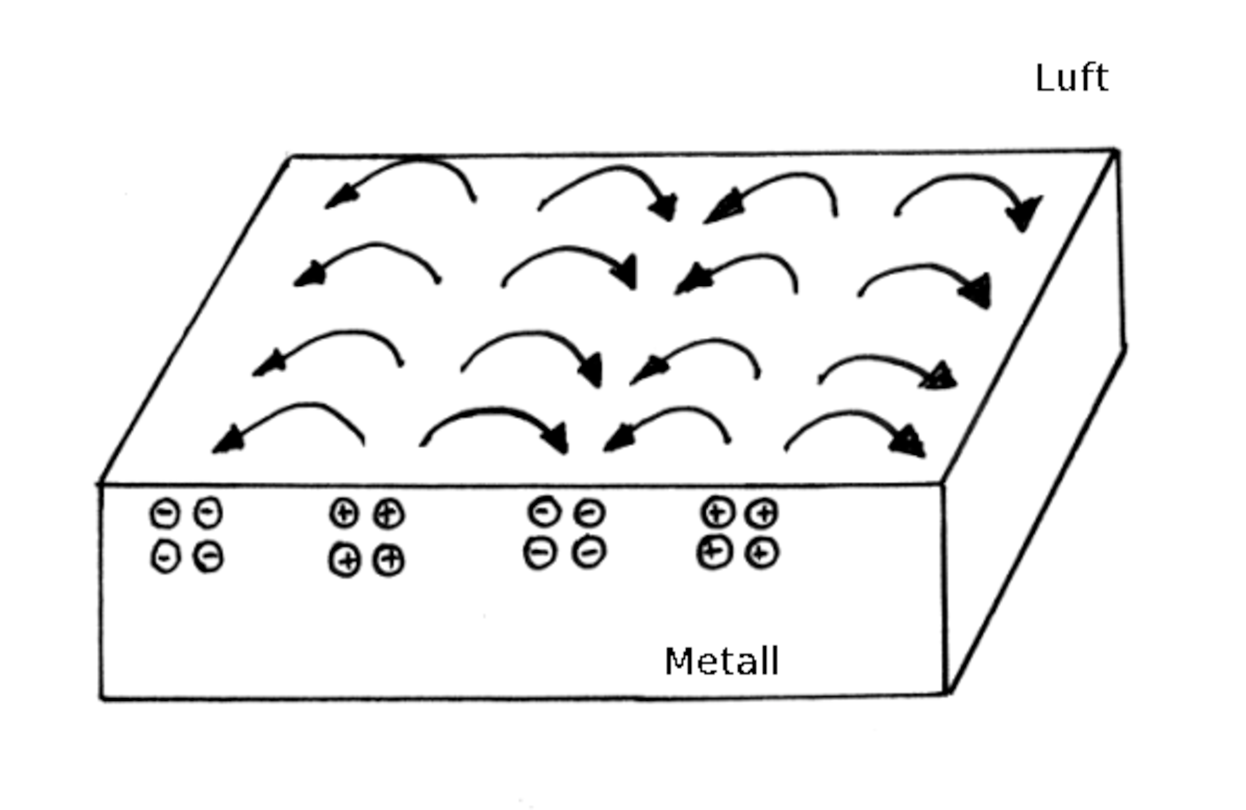
\includegraphics[width=0.8\textwidth]{op-.pdf}
	\caption{Oberfl�chenplasmonen in der Grenzschicht zwischen Metall und Luft}
	\label{fig:op}
\end{figure}

Es gibt dann potentiell Anregungen von Oberfl�chenplasmonen durch
bez�glich seiner Einfallsebene zur Grenzfl�che
$p$-polarisiertem Licht, mit einem $k_\text{OP}$--Vektor gleich der zur Grenzfl�che
parallelen Komponente des $k$--Vektors von Licht. Die Resonanzen dieser Anregung
geschehen bei �bereinstimmung von sowohl Frequenz $\omega$ als auch Wellenl�nge
$\frac{2\pi}{k}$ des zur Grenzfl�che
parallelen Anteils des Lichts und der Oberfl�chenplasmonen, also bei Schnittpunkten
der jeweiligen Dispersionrelationen zwischen $\omega$ und $k$.

\section{Dispersionsrelationen} \label{sec:disprel}

Die Dispersionsrelation von Oberfl�chenplasmonen in der Grenzschicht zwischen einem
Metall (2) mit Permittivit�t $\eps_2$ und einem Dielektrikum (1) mit Permittivit�t
$\eps_1$ ist
\begin{equation}	\label{eq:opdisp}
	k = \frac{\omega}{c}\sqrt{\frac{\eps_1\eps_2}{\eps_1+\eps_2}}
\end{equation}

Die Dispersionsrelation von Licht in einem Dielektrikum ($i$) mit Permittivit�t $\eps_i$
ist
\begin{equation}
	k = \frac{\omega}{c}\sqrt{\eps_i}
\end{equation}

Wenn Licht mit Einfallswinkel $\theta$ auf eine ebene Grenze des Dielektrikums $(i)$ f�llt,
dann gilt damit f�r die
zur Ebene parallele Komponente $k_x$ des Licht--$k$--Vektors
\begin{equation}	\label{eq:lichtprojdisp}
	k = \frac{\omega}{c}\sqrt{\eps_i}\sin{\theta}
\end{equation}

\section{Permittivit�ten} \label{sec:perm}

Die Permittivit�t von Luft ist in guter N�herung 1.

F�r die Permittivit�t von Glas gibt es die empirische N�herungsformel

\begin{equation}
	\eps_\text{Glas}
	= 2,979864 + \frac{877780,8}{\frac{\lambda}{\mathring{A}}^2-1060900}
	- \frac{84,06224}{96-\frac{\lambda}{\mathring{A}}^2 10^{-8}}
\end{equation}

und f�r Silber haben wir

\begin{equation}
	\begin{split}
	\eps_\text{Ag}
	= &-219,945 - 0,0261695\frac{\lambda}{\mathring{A}}
	+ 3,8559 \sqrt{\frac{\lambda}{\mathring{A}}}
	+ \frac{4857,2}{\sqrt{\frac{\lambda}{\mathring{A}}}} \\
	&+ i(7,139 + 0,001656\frac{\lambda}{\mathring{A}}
	- 0,2129 \sqrt{\frac{\lambda}{\mathring{A}}})
	\end{split}
\end{equation}

\section{} %\label{sec:experimentelle_methoden}

Es gibt keine Schnittpunkte der Dispersionsrelationen von Oberfl�chenplasmonen
und dem zur Oberfl�che parallelen Anteil von Licht bei der Grenzfl�che zwischen
einem Metall und einem Dielektrikum. Daher k�nnen auf diese Weise durch auf 
Metall schr�g einfallendes Licht keine Oberfl�chenplasmonen angeregt werden.

Es gibt jedoch Schnittpunkte zwischen den Dispersionsrelationen des parallelen Anteils
von Licht in Glas zu einer Grenzfl�che zu Silber und von Oberfl�chenplasmonen in der
Grenzschicht zwischen Silber und Luft. Dies kann mithilfe des Effekts der
frustrierten Totalreflexion f�r die Anregung von Oberfl�chenplasmonen durch Licht
ausgenutzt werden.

Licht wird an einer Grenzfl�che von Glas zu Silber totalreflektiert. Auf eine sehr d�nne
Silberschicht folgt eine Grenzfl�che zu Luft, an der ein nichtverschwindender Anteil der
evaneszenten Welle von der Totalreflexion �brig bleibt und Oberfl�chenplasmonen in
der Silber-Luft-Grenze anregen. Hier sind also Schnittpunkte der Dispersionsrelationen
des parallelen Anteils
von Licht in Glas zur Grenzfl�che zu Silber und von Oberfl�chenplasmonen in der
Silber-Luft-Grenze gesucht.



Die Reflektivit�t an der Glas-Silber-Luft-Schicht ist
\begin{equation}
	
\end{equation}
\chapter{Versuchsaufbau und -durchf�hrung}
\begin{figure}[ht]
    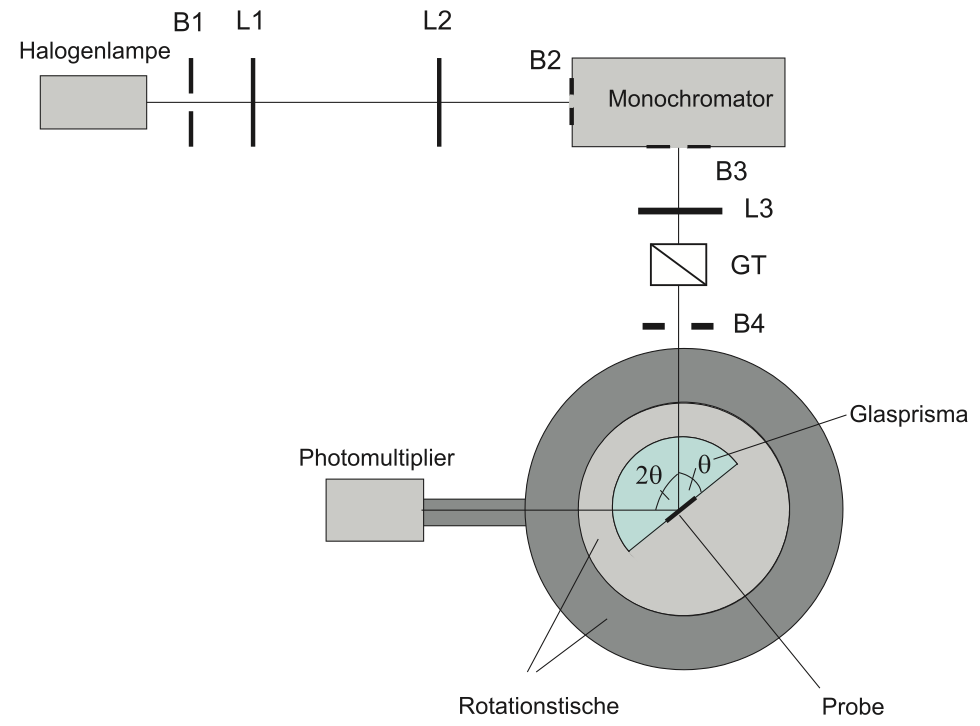
\includegraphics[width=1\textwidth]{op-aufbau.png}
	\caption{Aufbau zur Untersuchung der Oberfl�chenplasmonen}
	\label{fig:opaufbau}
\end{figure}
In diesem Versuch m�chten wir eine Probe mit $p$-polarisiertem monochromatischem
Licht bei variierendem Winkel bestrahlen und dabei den Aufbau so konstruieren,
dass die Wellenl�nge des Lichtes als Parameter sich auch leicht �ndern l�sst. 

Dazu verwenden wir eine Halogenlampe, dessen Licht wir durch eine Blende und
zwei Linsen in einen Monochromator lenken. Die Lampe emittiert ein weites,
kontinuierliches Spektrum an Licht. Im Monochromator wird das Licht in einem 
frequenzabh�ngigen Winkel an einem Gitter gebeugt und durch einen Spalt geschickt.

Das Licht wird dann polarisiert und trifft auf das Glasprisma und die Probe,
wo es die Plasmonen anregen soll. Ein Teil des Lichtes wird auf einen Photomultiplier
reflektiert, wo seine Intensit�t gemessen wird. 

Die Probe ist zusammen mit dem Glasprisma und dem Photomultiplier auf einem
Rotationstisch befestigt. Diesen kann man manuell oder motorisiert bedienen
und damit den Winkel, mit dem das Licht auf die Probe und in den Multiplier reflektiert wird,
abfahren.

Bevor wir mit der eigentlichen Untersuchung der Oberfl�chenplasmonen starten k�nnen,
m�ssen wir zuerst den Winkel des Rotationstisches kalibrieren.
Dazu nutzen wir den Effekt der Totalreflexion aus. Wir konstruieren den Aufbau ohne Probe und messen die Totalreflexion
am �bergang Glasprisma-Luft. Mit Licht einer bestimmten Wellenl�nge fahren wir einen Winkelbereich von ca. (10-50)� ab,
und vergleichen die gemessenen Werte f�r den Totalreflexionswinkel mit den Theoretischen.
Die Differenz zwischen den beiden Werten verwenden wir nun als Kalibrierungskonstante $\theta_0$.



\section{Oberfl�chenplasmonen auf einer glatten Probe}

Im ersten Versuchsteil arbeiten wir mit Silber-Proben, die eine vorgegebene
Schichtdicke von 20nm--70nm haben. Im ersten Durchgang arbeiten wir mit Licht
der Wellenl�nge 550 nm und variieren bei festen Schichtdicken den Einfallswinkel
und messen die Reflektivit�t.
Die Schichtdicke l�sst sich daraus berechnen, N�heres dazu ist in der Auswertung zu finden.


Um die Dispersionsrelation der Oberfl�chenplasmonen zu bestimmen, nehmen wir die
Probe mit dem tiefsten Absorptionsprofil und messen erneut die Relfektivit�t f�r verschiedene Winkel.

\section{Oberfl�chenplasmonen auf einer gittermodulierten Probe}

Bei der Untersuchung der gittermodulierten Probe  bestimmen wir zun�chst die Gitterkonstante.
Dazu nutzen wir die Beugung am Gitter aus.
Mit einem Laser bestrahlen wir die Probe unter einem senkrechten Winkel und
messen den Winkel zwischen den Beugungsmaxima 0. und 1. Ordnung.

In der eigentlichen Messung verwenden wir die Gitter-Probe, wobei der �brige Aufbau
bis auf das Glasprisma, das nun nicht ben�tigt wird, gleich bleibt.
Zur Justage der Gitterprobe kann man die Beugungseffekte ausnutzen,
um die Richtung der Gitterperiodizit�t in die Ebene des Aufbaus einzustellen.

Wir w�hlen einen Messbereich von 475nm--625nm f�r die Wellenl�nge und variieren
jeweils wieder den Einfallswinkel und messen die Reflektivit�t.
\chapter{Auswertung}

\section{Winkelkalibrierung}

Wir messen am Rotationstisch jeweils den Winkel $\alpha$, der mit dem wahren
Einfallswinkel $\theta$ des Lichts auf die Probe wie folgt zusammenh�ngt:
\begin{equation}
	\alpha = 2 \theta + \theta_0
\end{equation} \label{eq:kali}
wobei $\theta_0$ die Kalibrierungskonstante ist, die hier zu bestimmen ist.

Dies geschieht, indem wir experimentell den Wert f�r $\alpha$ suchen,
an dem Totalreflexion stattfindet
und diesen mit dem theoretischen Totalreflexionswinkel $\theta_\text{tot}$ nach
Gleichung \eqref{eq:totref} �ber \eqref{eq:kali} Verbindung bringen.

Um den Totalreflexionswinkel experimentell zu bestimmen, haben wir f�r verschiedene
Wellenl�ngen von 500nm -- 600nm einen gro�en Winkel zwischen 0 und 90 Grad bez�glich des
einfallenden Lichtstrahles abgefahren und die Reflektivit�t des Glasprismas unter
diesem Winkel gemessen.

Wir erwarten einen stufenf�rmigen Verlauf, wobei die Reflektivit�t bei 0 anf�ngt,
an dem Totalreflexionswinkel auf 1 springt und bis 90 Grad weiterverl�uft. 

Dies ist eine idealisierte Betrachtungsweise. Wir werden im Experiment eine stetige
Kurve an der Totalreflexionsstelle sehen
und versuchen f�r jeden Messdurchlauf diese Stelle mit zwei Geraden anzufitten.

\begin{figure}[ht]
    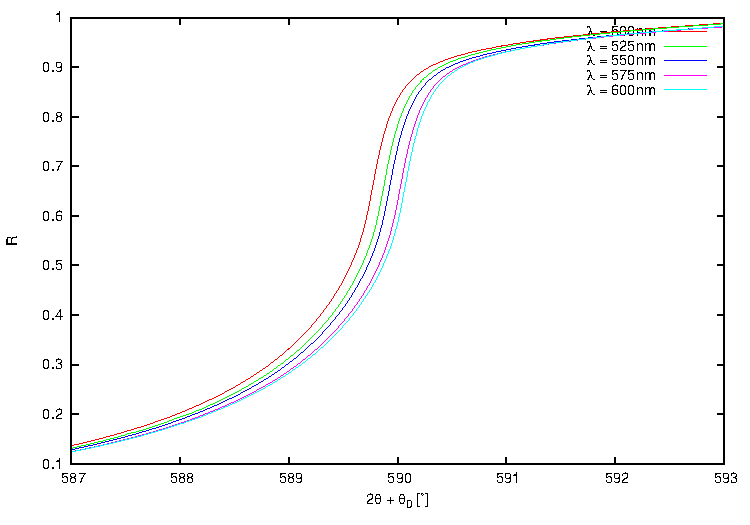
\includegraphics[width=1\textwidth]{totalreflexionen.pdf}
	\caption{Gemessene Reflektivit�ten $R$ in Abh�ngigkeit der zu kalibrierenden
	  	   		Winkelangabe des Rotationstisches $2\theta+\theta_0$ bei verschiedenen
				Wellenl�ngen $\lambda$ einfallenden Lichts.}
	\label{fig:totref}
\end{figure}

\begin{figure}[h]
    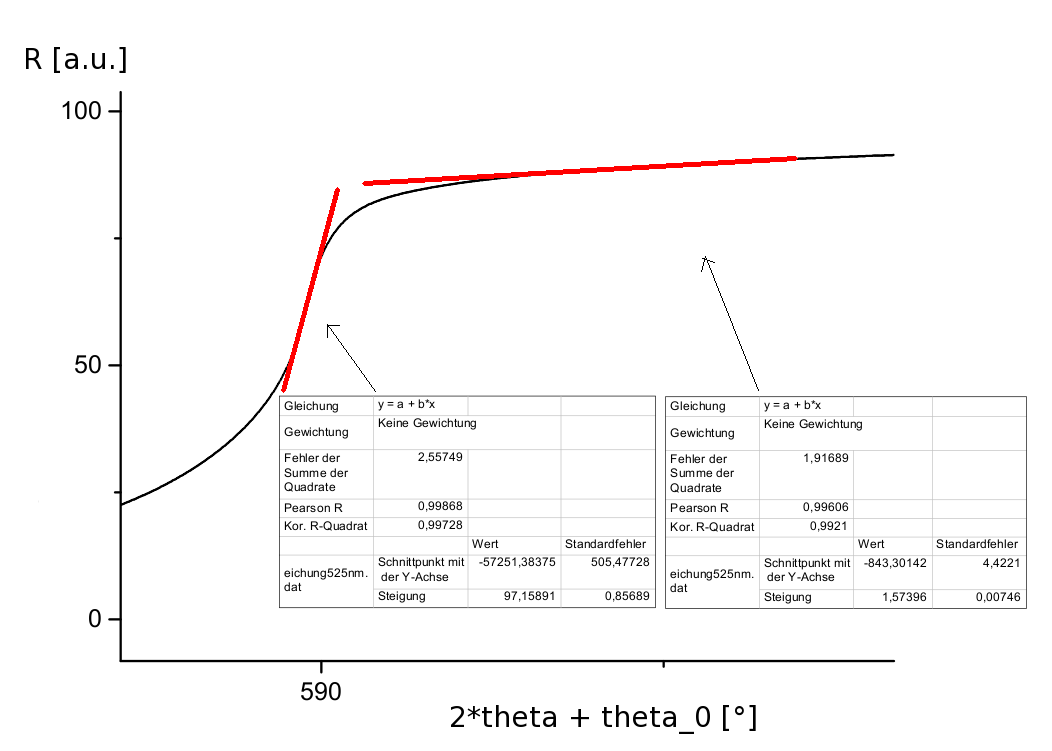
\includegraphics[width=1\textwidth]{linreg-totref-525nm.png}
	\caption{Gemessene Reflektivit�t $R$ in Abh�ngigkeit der zu kalibrierenden Winkelangabe
				des Rotationstisches $(2\theta+\theta_0)$ bei Wellenl�nge
				$\lambda=525\text{nm}$. In Rot die linearen Regressionen
				zur Bestimmung des Totalreflexionswinkels.}
	\label{fig:linreg}
\end{figure}

Wie man in Abbildung \ref{fig:totref} sehen kann, verschiebt sich die Kurve bei h�heren
Wellenl�ngen in Richtung gr��eren Winkeln, was mit 
der Frequenzabh�ngigkeit der Permittivit�t von Glas $\eps_\text{Glas}(\lambda)$ zusammenh�ngt.

In Abbildung \ref{fig:linreg} sieht man ein Beispiel f�r den Fit, den wir an allen f�nf
Messkurven durchgef�hrt haben. In Tabelle \ref{tab:totref} sieht man nun
die eingestellten Wellenl�ngen, den theoretischen Wert $\theta_\text{tot}$ und experimentellen
Wert $\alpha_\text{tot}$ f�r die Totalreflexion, sowie den errechneten Offset $\theta_{0}$.

\begin{table}[h]
	\centering
\begin{tabular}[t]{|l|l|l|l|}

\hline
$\lambda$ [nm]& $\theta_\text{tot}$ [�] & $\alpha_\text{tot}$ [�] &$\theta_{0}$ [�] \cellcolor{dunkelgrau} \\
\hline
500 & 43,14 &590,05 &503,77\cellcolor{dunkelgrau}\\
\hline
525 & 43,19 &590,10 &503,72\cellcolor{dunkelgrau}\\
\hline
550 & 43,23 &590,19 &503,73\cellcolor{dunkelgrau}\\
\hline
575 & 43,27 &590,30 &503,76\cellcolor{dunkelgrau}\\
\hline
600 & 43,30 &590,19 &503,73\cellcolor{dunkelgrau}\\
\hline
\end{tabular}\caption{Winkelangabe $\alpha_\text{tot}$ des
	 	Rotationstisches bei Totalreflexion, Kalibrierungskonstante $\theta_{0}$
		bez�glich des theoretischen Totalreflexionswinkels und der damit berechnete
		gemessene Totalreflexionswinkel $\theta_\text{tot}$.} \label{tab:totref}
\end{table}

Die mittlere Kalibrierungskonstante, die wir ab nun ber�cksichtigen werden, lautet dann:
$\theta_{0}= (503,74 \pm 0,02)$�
\clearpage

\section{Oberfl�chenplasmonen in glatten Silberfilmen}

\subsection{Verschiedene Probendicken}

\begin{figure}[!h]
    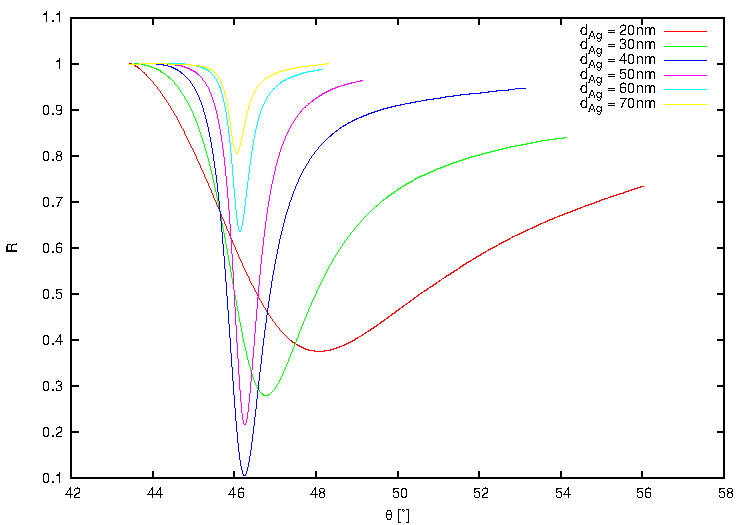
\includegraphics[width=1\textwidth]{ag-dicken.pdf}
	\caption{Gemessene Reflektivit�ten $R$ in Abh�ngigkeit des Einfallswinkels
				$\theta$ bei verschiedenen Ag-Probendicken $d$.}
	\label{fig:agdicken}
\end{figure}

In Abbildung \ref{fig:agdicken} sind unsere Messdaten der Reflektivit�ten bei verschiedenen
Dicken $d$ der Silberschicht dargestellt. Die Wellenl�nge $\lambda$ ist jeweils 550nm.

Mithilfe der Gleichungen \eqref{eq:r012}, \eqref{eq:permiag}, \eqref{eq:permiglas} und
\eqref{eq:lichtprojdisp} kann die Reflektivit�t $R$ als Funktion des Einfallswinkels
$\theta$ in Abh�ngigkeit des Parameters $d$ auch theoretisch berechnet werden.
F�r jede der sechs Silberproben verschiedener Dicke machen wir einen Fit dieser
Funktion an die Messdaten zur Bestimmung des Parameters $d$. Die Ergebnisse sind
in Tabelle \ref{tab:agdicken} dargestellt.

\begin{table}[h]
\centering
\begin{tabular}{| >{$}c<{$} >{$}c<{$} |}
\hline
d_\text{nom}\text{ [nm]}		&	 d\text{ [nm]}	\\ [0.2ex]
\hline\hline
20		&		20,00			\\
30		&		30,89			\\
40		&		42,66			\\
50		&		62,44			\\
60		&		78,60			\\
70		&		87,54			\\
\hline
\end{tabular}
\caption{Angegebene Probendicken $d_\text{nom}$ und
			experimentell bestimmte Probendicken $d$}	\label{tab:agdicken}
\end{table}

F�r gr��ere Schichtdicken weichen die von uns ermittelten Werte zunehmend von Werten, die
auf den Packungen der Proben standen, ab.
An den Silberproben waren viele schwarze Flecke zu sehen, die auf eine starke Oxidation der
Probe hinweist. Da wir die vierte Gruppe waren,
die diese Probe verwendet haben, k�nnte eine starke Verschmutzung die Abweichung der Schichtdicke
vom angegebenen Wert erkl�ren. 

\subsection{Permittivit�t von Silber}

In Abbildung \ref{fig:festeagdicke} sind unsere Messdaten der Reflektivit�ten bei
verschiedenen Wellenl�ngen $\lambda$ des reflektierten Lichts und fester Probendicke
$d=40$nm dargestellt.

\begin{figure}[ht]
    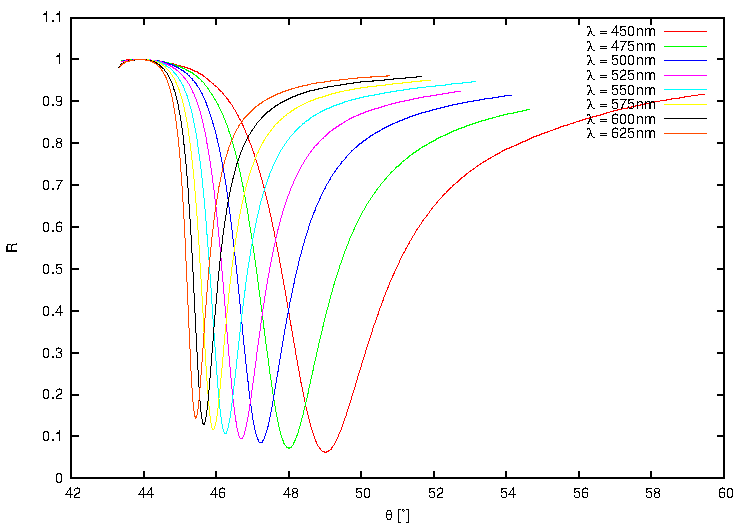
\includegraphics[width=1\textwidth]{feste-ag-dicke.pdf}
	\caption{Gemessene Reflektivit�ten $R$ in Abh�ngigkeit des Einfallswinkels
				$\theta$ bei verschiedenen Wellenl�ngen $\lambda$ einfallenden
				Lichts.}
	\label{fig:festeagdicke}
\end{figure}

\begin{figure}[h]
	\subfigure[Realteil der Permittivit�t]{
    	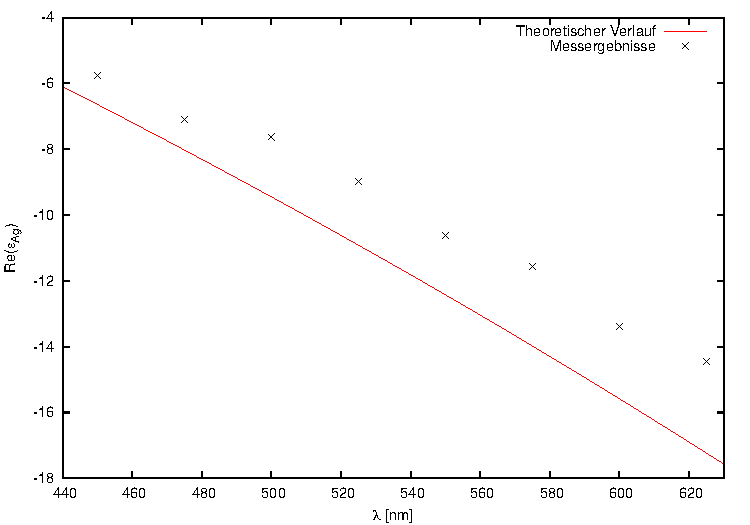
\includegraphics[width=0.5\textwidth]{permi-re.pdf}
	}
	\subfigure[Imagin�rteil der Permittivit�t]{
    	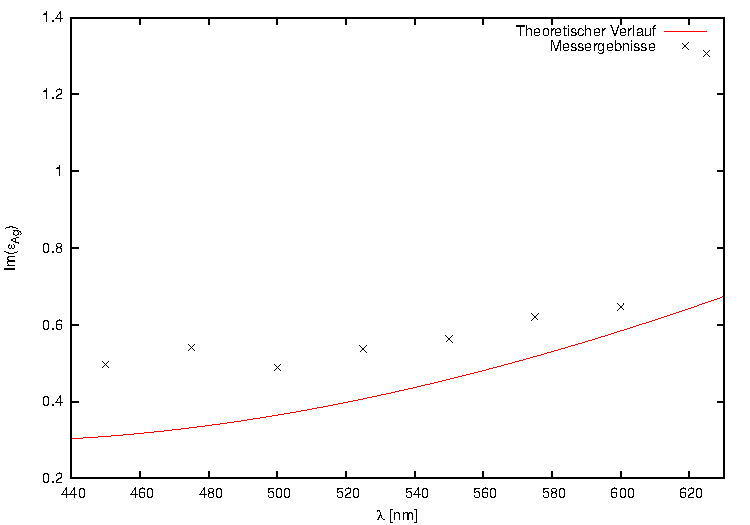
\includegraphics[width=0.5\textwidth]{permi-im.pdf}
	}
	\caption{Experimentell bestimmte Werte f�r $\eps_\text{Ag}$ zu verschiedenen
			Wellenl�ngen $\lambda$ und der theoretische Verlauf
				$\lambda \mapsto \eps_\text{Ag}$.}
	\label{fig:permitti}
\end{figure}

Mithilfe der Gleichungen \eqref{eq:r012}, \eqref{eq:permiag}, \eqref{eq:permiglas} und
\eqref{eq:lichtprojdisp} kann die Reflektivit�t $R$ wieder als Funktion des Einfallswinkels
$\theta$, diesmal jedoch in Abh�ngigkeit des komplexen Parameters $\eps_\text{Ag}$
theoretisch berechnet werden. Wir machen also f�r jede Messung mit einer bestimmten
Wellenl�nge einen Fit dieser Funktion an die Messdaten zur Bestimmung der Parameter
$\Re (\eps_\text{Ag})$ und $\Im (\eps_\text{Ag})$.
Au�erdem kennen wir mit der N�herungsformel \eqref{eq:permiag} die theoretischen
Verl�ufe von $\lambda \mapsto \Re (\eps_\text{Ag})$ und
$\lambda \mapsto \Im (\eps_\text{Ag})$.\\
Sowohl die experimentellen Ergebnisse als auch der theoretische Verlauf sind in Abbildung
\ref{fig:permitti} dargestellt.

Man erkennt eine gewisse korrelierte Abweichung der Messpunkte von der theoretischen
Kurve, was auf einen systematischen Fehler hindeutet. Dieser k�nnte durch
Verunreinigung oder Oxidation der verwendeten Probe verursacht sein.
\clearpage

\subsection{Dispersionsrelation}

Die Minima der Reflektivit�t in den Messkurven in Abbildung \ref{fig:festeagdicke}
entsprechen den Resonanzen der Oberfl�chenplasmonen. Wir gehen also davon aus,
dass die entsprechende Kombination von Einfallswinkel $\theta$ und Wellenl�nge
$\lambda$ des einfallenden Lichts, die mit \eqref{eq:lichtprojdisp} einer Kombination
von Impuls $k$
und Kreisfrequenz $\omega$ der Oberfl�chenplasmonen entspricht,
ein Punkt der Dispersionsrelation der Plasmonen ist.

\begin{figure}[!h]
    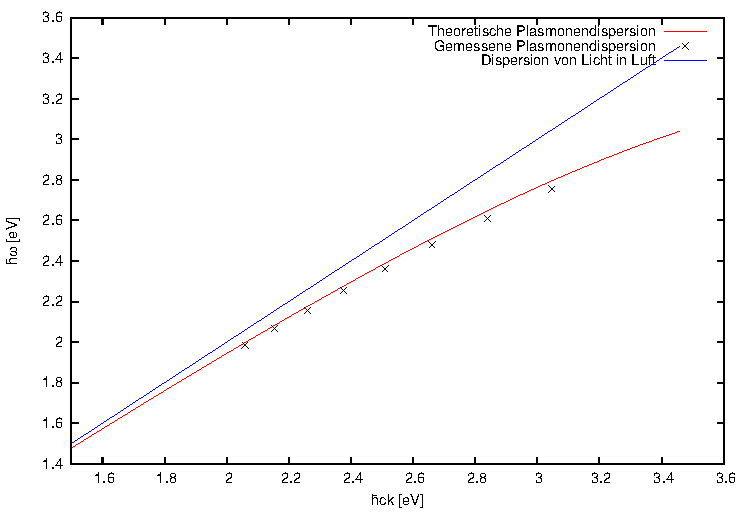
\includegraphics[width=1\textwidth]{glattdisp.pdf}
	\caption{Experimentell bestimmte Punkte und theoretischer Verlauf der
				Oberfl�chenplasmonendispersion.}
	\label{fig:glattdisp}
\end{figure}

Die so experimentell bestimmten Punkte der Oberfl�chenplasmonendispersion sind
in Abbildung \ref{fig:glattdisp} zusammen mit dem theoretischen Verlauf nach
\eqref{eq:opdisp} dargestellt.

\clearpage

\section{Oberfl�chenplasmonen in einer gittermodulierten Silberprobe}

F�r die Gitterkonstante der Probe erhalten wir $a=698$ nm, womit wir f�r die Oberfl�chenplasmonen
eine Brillouinzonengr��e von $1,776\ \frac{\text{eV}}{\hbar c}$ erwarten.

Wie oben erhalten wir aus den Minima der Reflektivit�ten bei verschiedenen Wellenl�ngen
einfallenden Lichts einzelne Punkte des Dispersionsgraphen, welche in Abbildung
\ref{fig:gitterdisp} zusammen mit der theoretischen Dispersionrelation (zum Teil um reziproke
Gittervektoren zur�ck- bzw. vorgefaltet) dargestellt sind.

\begin{figure}[!h]
    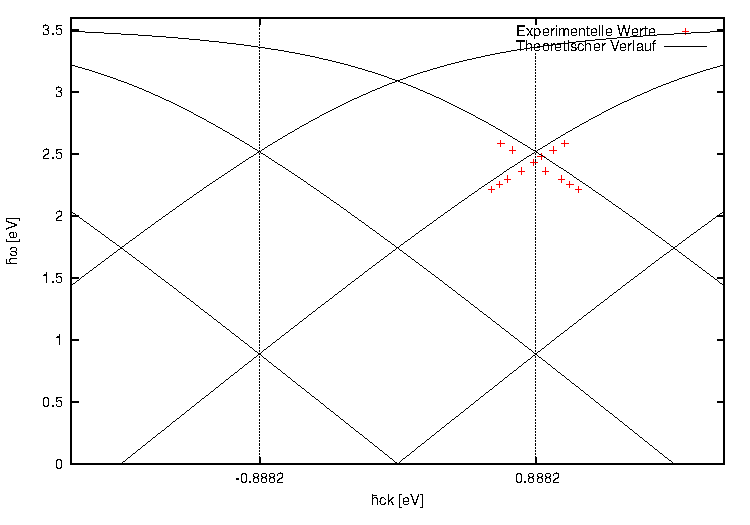
\includegraphics[width=1\textwidth]{gitterdisp.pdf}
	\caption{Experimentell bestimmte Punkte und theoretischer Verlauf der
				Oberfl�chenplasmonendispersion in der gittermodulierten Probe.
				Gestrichelt dargestellt ist der Brillouinzonenrand ermittelt aus der
				gemessenen Gitterkonstanten.}
	\label{fig:gitterdisp}
\end{figure}

Man kann sehen, dass es hier, �hnlich wie oben, eine leichte korrelierte Abweichung der
experimentellen Werte von
den theoretischen gibt. Bei unseren Berechnungen sind wir von einer Gitterprobe bestehend aus einer
Silberschichtgitterstruktur ausgegangen und haben dementsprechend
die Permittivit�ten von Silber und Luft verwendet. Zur vereinfachten Produktion wurde aber ein
Kunststoff verwendet, der nat�rlich eine Abweichung in 
der Permittivit�t hervorruft und damit auch eine systematische Fehlerquelle in den Messungen sein
kann.
\chapter{}
\section{}

% Literaturverzeichnis mit File literatur.tex
\chapter{Literaturverzeichnis}



\end{document}

